\documentclass[10pt]{article}
\usepackage[utf8]{inputenc}
\usepackage{hyperref}
\usepackage{fontenc}
\usepackage{mathptmx}
\usepackage{geometry}
\usepackage{titling}
\usepackage{graphicx}
\usepackage{subcaption}


\usepackage[noend]{algorithmic}
\newcommand{\TITLE}[1]{\item[#1]}
\renewcommand{\algorithmiccomment}[1]{$/\!/$ \parbox[t]{4.5cm}{\raggedright #1}}
% ugly hack for for/while
\newbox\fixbox
\renewcommand{\algorithmicdo}{\setbox\fixbox\hbox{\ {} }\hskip-\wd\fixbox}


\setlength{\topskip}{0mm}
\setlength{\droptitle}{-8em} 
\title{{\large \textbf{CONCORDIA UNIVERSITY \\ DEPARTMENT OF COMPUTER SCIENCE AND SOFTWARE ENGINEERING \\ SOEN 6011: SOFTWARE ENGINEERING PROCESSES \\ SECTION CC WINTER 2019 \\ F1: $arccos(x)$}  \\ }}
\author{\normalsize \textbf {STUDENT NAME: YONGCONG LEI} \\ \normalsize \textbf{STUDENT IDENTIFICATION NUMBER: 40045701 }}
\date{}
\begin{document}
\maketitle

\section{Characteristics and Domain}
\subsection{Characteristics}

\begin{enumerate}
    \item $arccos(x)$ is an inverse trigonometric function (relate an angle of a right-angled triangle to ratios of two side lengths), and it's tightly related to the trigonometric cosine function.
    
    \begin{figure}[h!]
      \centering
      \begin{subfigure}[b]{0.4\linewidth}
        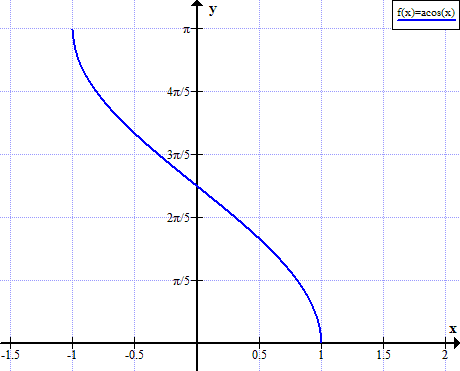
\includegraphics[width=\linewidth]{image/arccos.png}
        \caption{$arccos(x)$}
      \end{subfigure}
      \begin{subfigure}[b]{0.4\linewidth}
        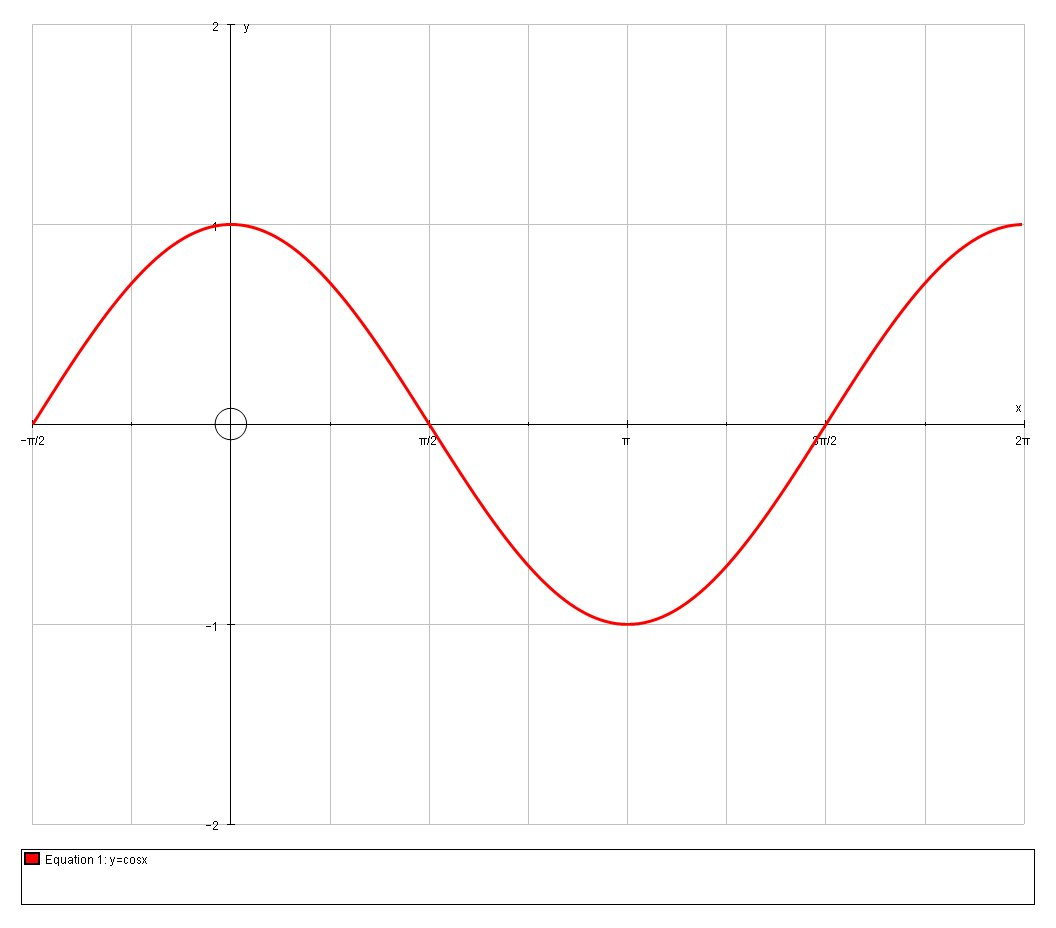
\includegraphics[width=\linewidth]{image/cos.jpg}
        \caption{$cos(x)$}
      \end{subfigure}
      \caption{$arccos(x)$ and $cos(x)$}
      \label{fig:coffee}
    \end{figure}

    
    \item $arccos(x)$ is an inverse trigonometric functions of $cos(x)$. In order introduce inverse trigonometric functions, we first need to take a look at trigonometric functions. In mathematics, the trigonometric functions are real functions which relate an angle of a right-angled triangle to ratios of two side lengths\cite{einstein}. $cos(x)$ is one of them. Given $$x = cos(y) = \frac{b}{h} = \frac{adjacent}{hypotenuse}$$ then $$y = arccos(x)$$ Figure 1 is an example of $cos(x)$. In this case, $x = cos(y) = \frac{OC}{OA}$. Therefore, $y = arccos(x) = arccos(\frac{OC}{OA})$.
    \begin{center}
      \begin{figure}[h!]
          \centering
          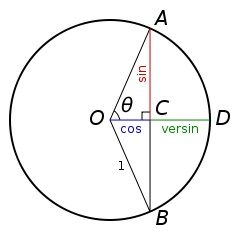
\includegraphics[width=0.3\linewidth]{image/cos_detail.jpg}
          \caption{trigonometric functions}
          \label{fig:my_label}
      \end{figure}
    \end{center}
    
    \item The function $arccos$ has their \textbf{principle values}. It's because inverse cosine function are not one-to-one.Therefore, the ranges of the inverse cosine functions are proper subsets of the domains of the original functions. With this restriction, for each x in the domain the expression $arccos$ will evaluate only to a single value, called its principal value. The range of principle values of $arccos(x)$ is $[-\frac{1}{2}\pi, \frac{1}{2}\pi]$. As a result, there will be one-to-one relationship for any value in domain.
\end{enumerate}

\subsection{Domain and Co-domain}
\paragraph{}
Since none of the six trigonometric functions are one-to-one, they are restricted in order to have inverse functions. The co-domain of $arccos(x)$ in area $[-\infty, \infty]$. However, we usually takes the principle values as its co-domain which is $[-\frac{1}{2}\pi, \frac{1}{2}\pi]$. Therefore, there will be one-to-one relationship between its domain and co-domain.

\paragraph{}
As a result, the domain is $x \in [-1, 1]$. The co-domain is $y \in [-\frac{1}{2}\pi, \frac{1}{2}\pi]$ for the equation $y = arccos(x)$.

\pagebreak
\section{Requirements}
\begin{enumerate}
    \item When a user apply a value $x \in [-1, 1]$ (which is the domain) to function $arccos(x)$, the calculator shall return a value $y\in [0, \pi]$.
    \item When a user apply a value $x \notin [-1, 1]$, the calculator shall show an error message.
    \item If the result is a infinite decimal, the result shall be shown to the nearest five decimal points.
    \item The calculator shall support input of operands such as digits or special irrational number such as $\pi, e$ etc.
    \item When a user enter anything to the calculator, the calculator shall show anything that user input.
    \item When a user input an invalid sequence of operands and operators, a error message shall be shown.
    \item When a user reset the calculator, all the ongoing transaction and history should be erased.
    \item The user shall be able to correct or modify his input to the calculator.
    \item The calculator shall be able to save the input sequence and related result to its memory.
\end{enumerate}

\pagebreak
\section{Algorithms}
\begin{enumerate}
    \item The algorithm uses the Lagrange Polynomial Approximation to calculate the arccos(x). The advantage of the algorithm is its performance. The time complexity is constant time. The advantage is that it has a maximum error of about 0.18 rad. Besides, The polynomial approximation performs pretty bad near $x=-1$ or $x=1$ where the derivative of the inverse cosine goes to infinity. Here is the pseudocode of the algorithhm. \newline
    
    \begin{algorithmic}[1]
      \TITLE{\textsc{Lagrange-polynomial-Approximation-arccos}$(x)$}
      \STATE $x\_square = x*x$
      \STATE $v1 = -0.69813170079773212 * x\_square - 0.87266462599716477$
      \STATE return $v1 * x + 1.5707963267948966$
    \end{algorithmic}

    \item Besides, there is an algorithm for $arccos(x)$ based on rational function - the quotient of two polynomials. The advantage is that it can give a a much better approximation. It has a maximum absolute error of 0.017 radians (0.96 degrees) on the interval (-1, 1). The disadvantage of the algorithm is that it involves division operator. In some cases, division is more expensive than addition and multiplication. Here is the pseudocode of the algorithm. \newline
    
    \begin{algorithmic}[1]
      \TITLE{\textsc{rational-function-Approximation-arccos}$(x)$}
      \STATE $a = -0.939115566365855$
      \STATE $b =  0.9217841528914573$
      \STATE $c = -1.2845906244690837$
      \STATE $d =  0.295624144969963174$
      \STATE $x\_square = x*x$
      \STATE $x\_cube = x\_square*x$
      \STATE $x\_quad = x\_cube*x$;
      \STATE return $(\pi / 2 + (a*x + b*x\_cube) / (1+ c*x\_square + d*x\_quad) )$
    \end{algorithmic}
\end{enumerate}

\begin{thebibliography}{9}
\bibitem{A comparison of rates of rational and polynomial approximation} 
E. P. Dolzhenko
\textit{A comparison of rates of rational and polynomial approximation}. 
Mathematical notes of the Academy of Sciences of the USSR, March 1967, Volume 1, Issue 3, pp 208–212

\bibitem{Rational values of the arccosine function} 
Juan L. Varona
\textit{Rational values of the arccosine function}. 
Central European Journal of Mathematics, June 2006, Volume 4, Issue 2, pp 319–322
\end{thebibliography}
 
\end{document}
